This section covers the empirical results using the methods mentioned earlier. Our interest lies in the aspects of accuracy, computation time and complexity, and for tests the errors of type I and II. 
\subsection{Accuracy}
The first point of interest is whether bootstrap techniques reach an acceptable level of accuracy. In this subsection we will assess this with the estimation of summary statistics (quantiles, mean and standard deviation). However, such a level of accuracy can be generalized easily without major drawbacks. Furthermore, we will adress the computation time of the bootstrap with respect to sample size and bootstrap iterations. Nonetheless, the computation time is not of much interest in such a setting and will be discussed more deeply in the following subsection. \\
As already mentioned, we measure accuracy with typical MSE and MAE. Figure~\ref{fig:summary} shows how MAE and MSE behave in estimating the mean of a sample using resampling methods. A complete table for summary statistics estimation can be found in Appendix A, see tables~\ref{tab:sum_mse_r},~\ref{tab:sum_mae_r},~\ref{tab:sum_mse_cpp} and~\ref{tab:sum_mae_cpp}. 

\begin{figure}
\centering
	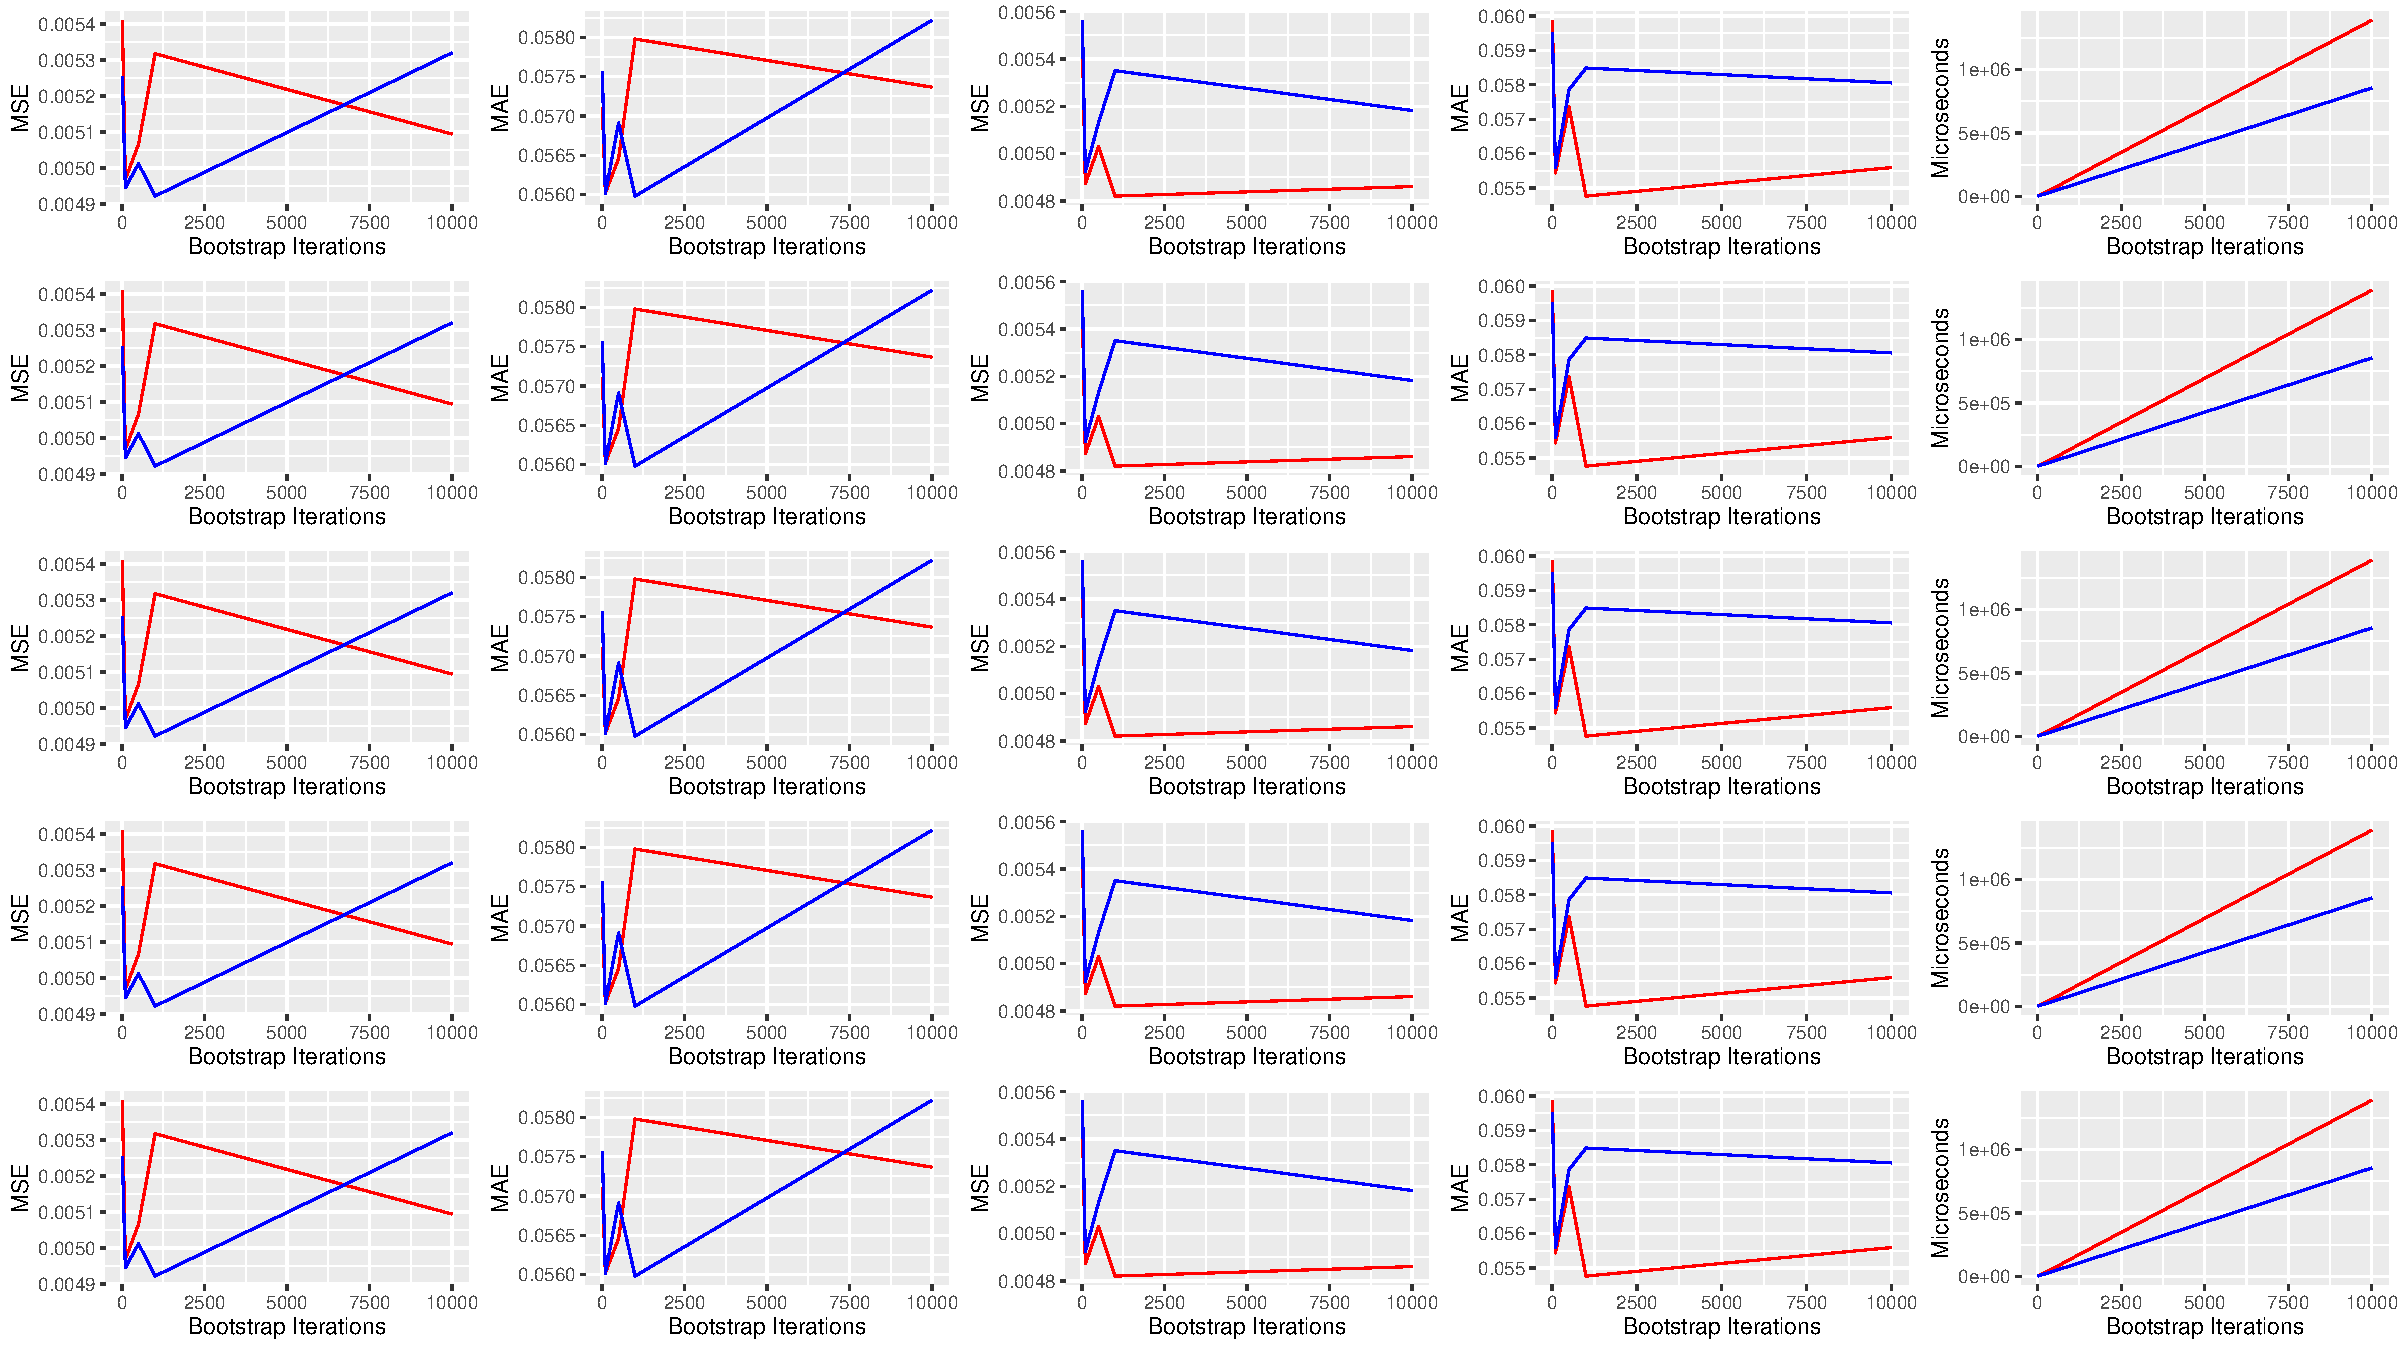
\includegraphics[scale=0.4]{./figures/plot_summary.pdf}
	\caption[Summary MSE and MAE]{Red Line: Nonparametric Bootstrap, Blue Line: Wild Bootstrap. Each row corresponds to a different number of sample size from ($5, 10, 50, 100, 200$), the first two columns correspond to the R-Version, whereas the third and fourth to the C++ version. The last column represents the median computation time (with red being the R and blue the C++ algorithm).}
	\label{fig:summary}
\end{figure}

\subsection{Computational Complexity}

In this subsection we want to adress one of the main advantages of C/C++. This is the speed of computations. Whereas R (or other languages such as python) are very high level languages which allow the user to do scientific analyses easily, lower level languages such as C and C++ offer a great advantage in speed for the cost of intuitiveness. To demonstrate such issues we present a simulated linear regression problem as mentioned in section~\ref{sec:sim}. In the following, we also show a figure of accuracy for the coefficients, although we used a different accuracy measure, namely the compound MSE and compound MAE as mentioned in the same section~\ref{sec:sim}. Since the accuracy is related to the accuracy of summary statistics and also dependent on the accuracy of the specific algorithm itself, there is not much additional error due to bootstrap (no systematic bias), see table~\ref{tab:regError} in Appendix B. 

\begin{figure}
\centering
	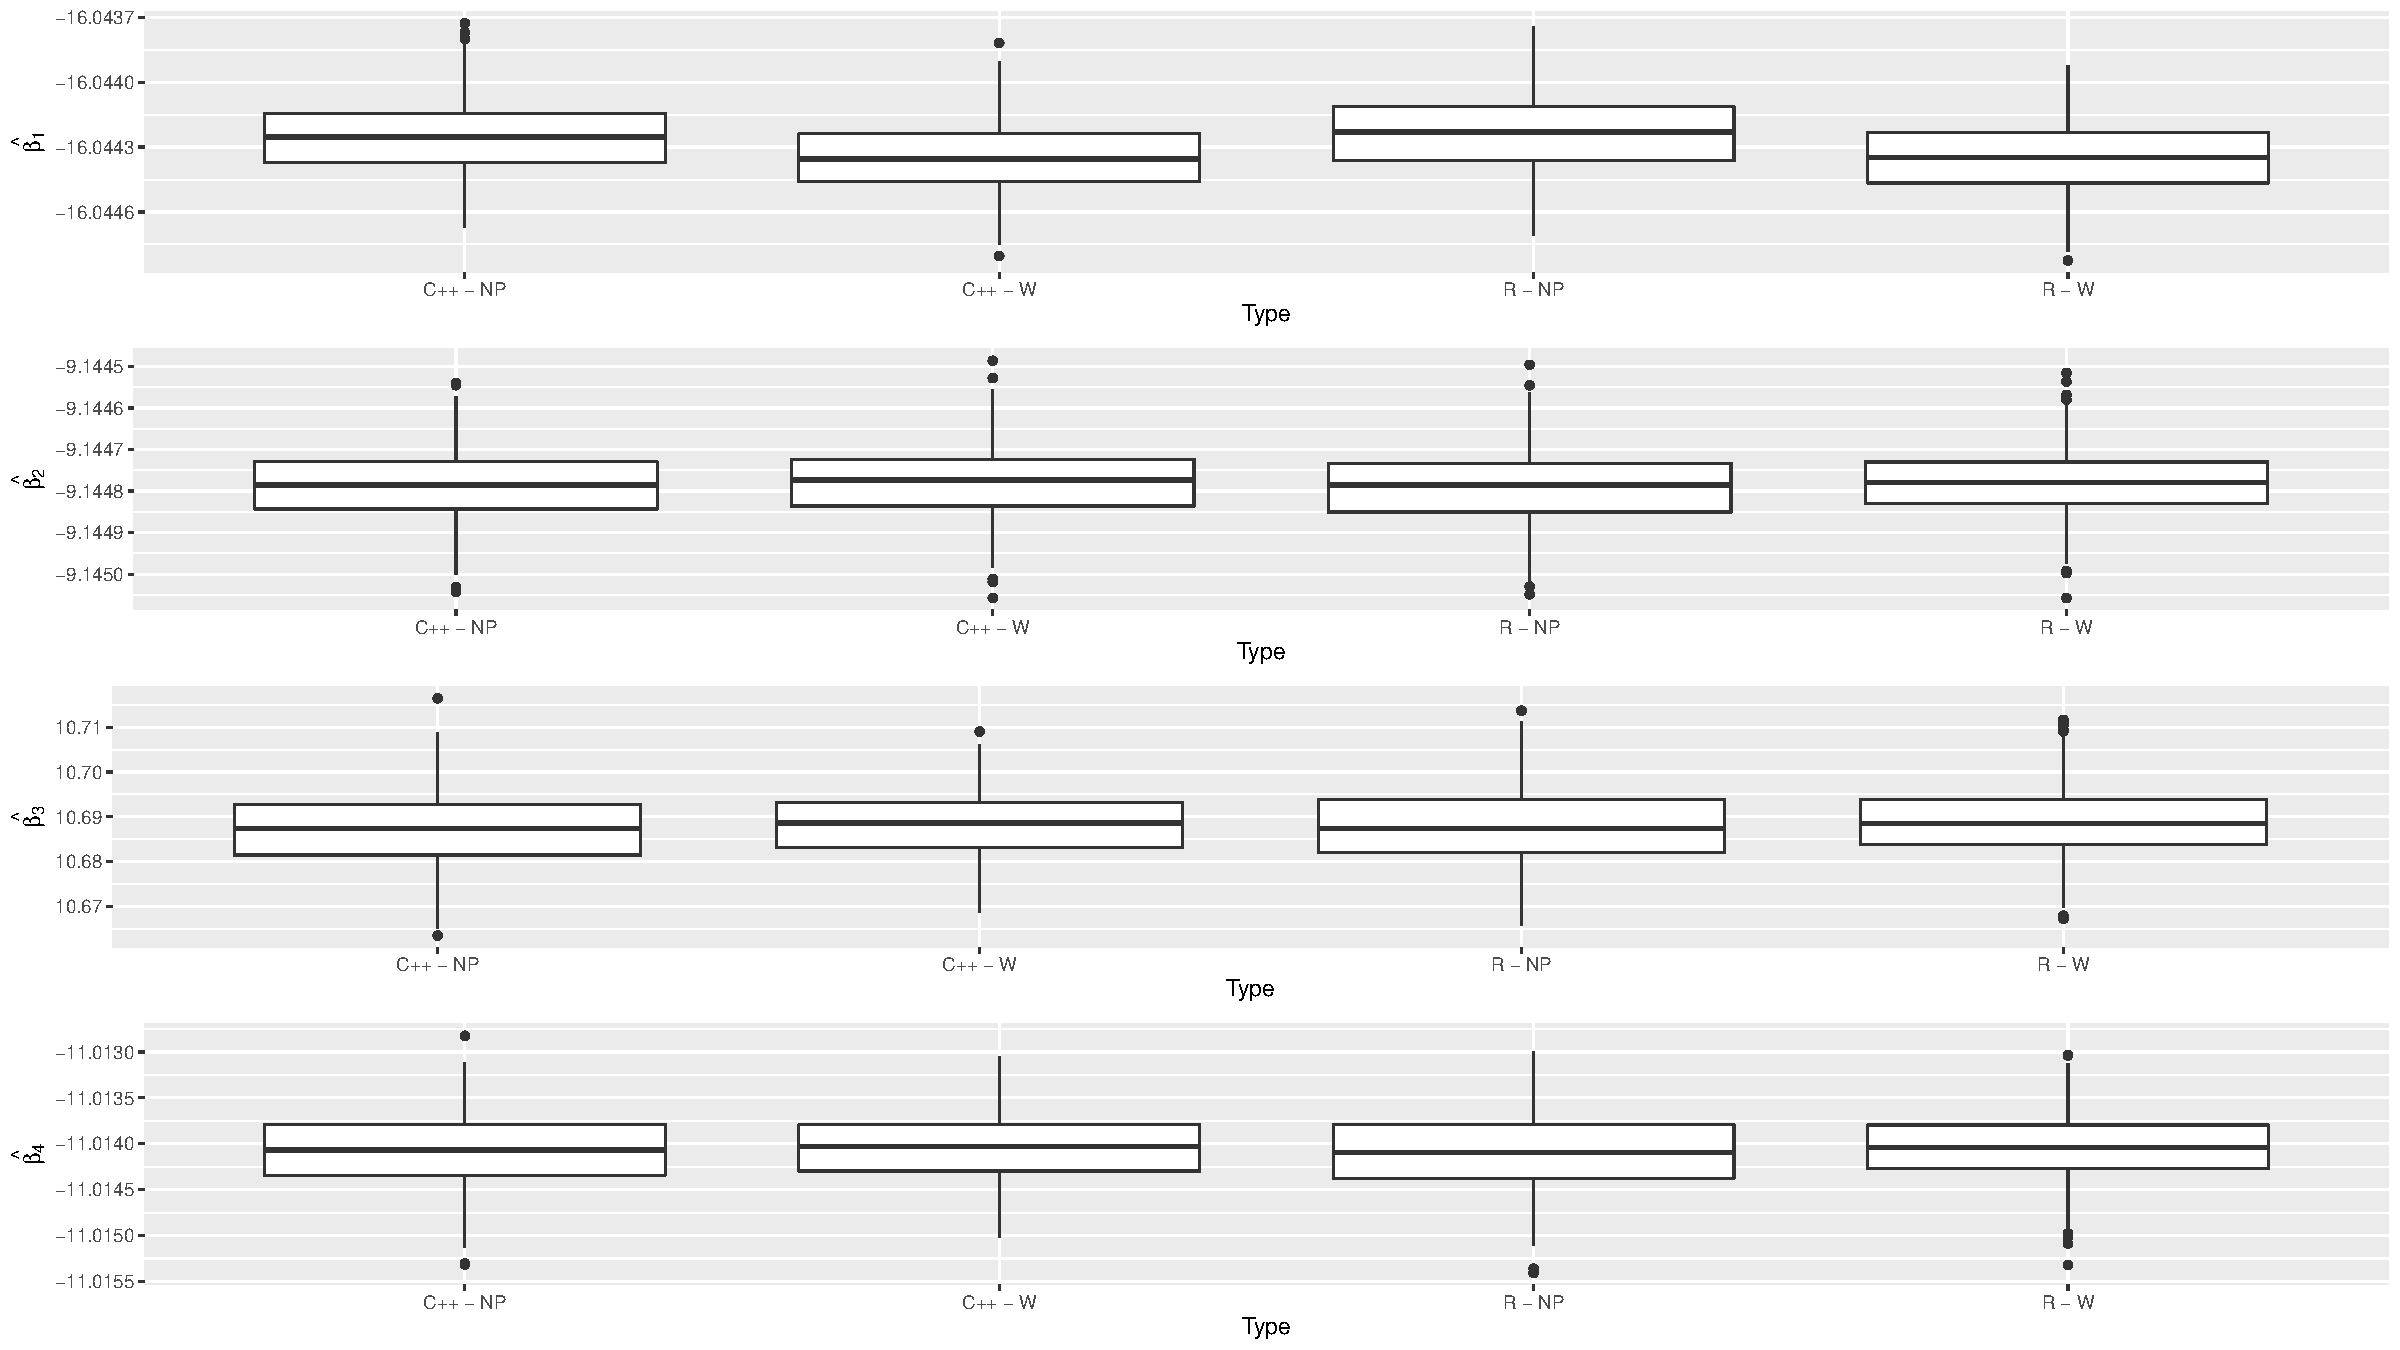
\includegraphics[scale=0.4]{./figures/plot_regression_error.pdf}
	\caption[Boxplot Coefficients]{Boxplot for all coefficients with respect to the bootstrap technique used}
	\label{fig:regErr}
\end{figure}

\noindent We see, that the estimated coefficients are quite close to the true coefficients. Also, we see that wild bootstrap provides slightly better results than nonparametric bootstrap. Since the origin of wild bootstrap is in regression analysis, this is not very surprising. However, the following plot shows how R and C++ differ in terms of computation time.

\begin{figure}
\centering
	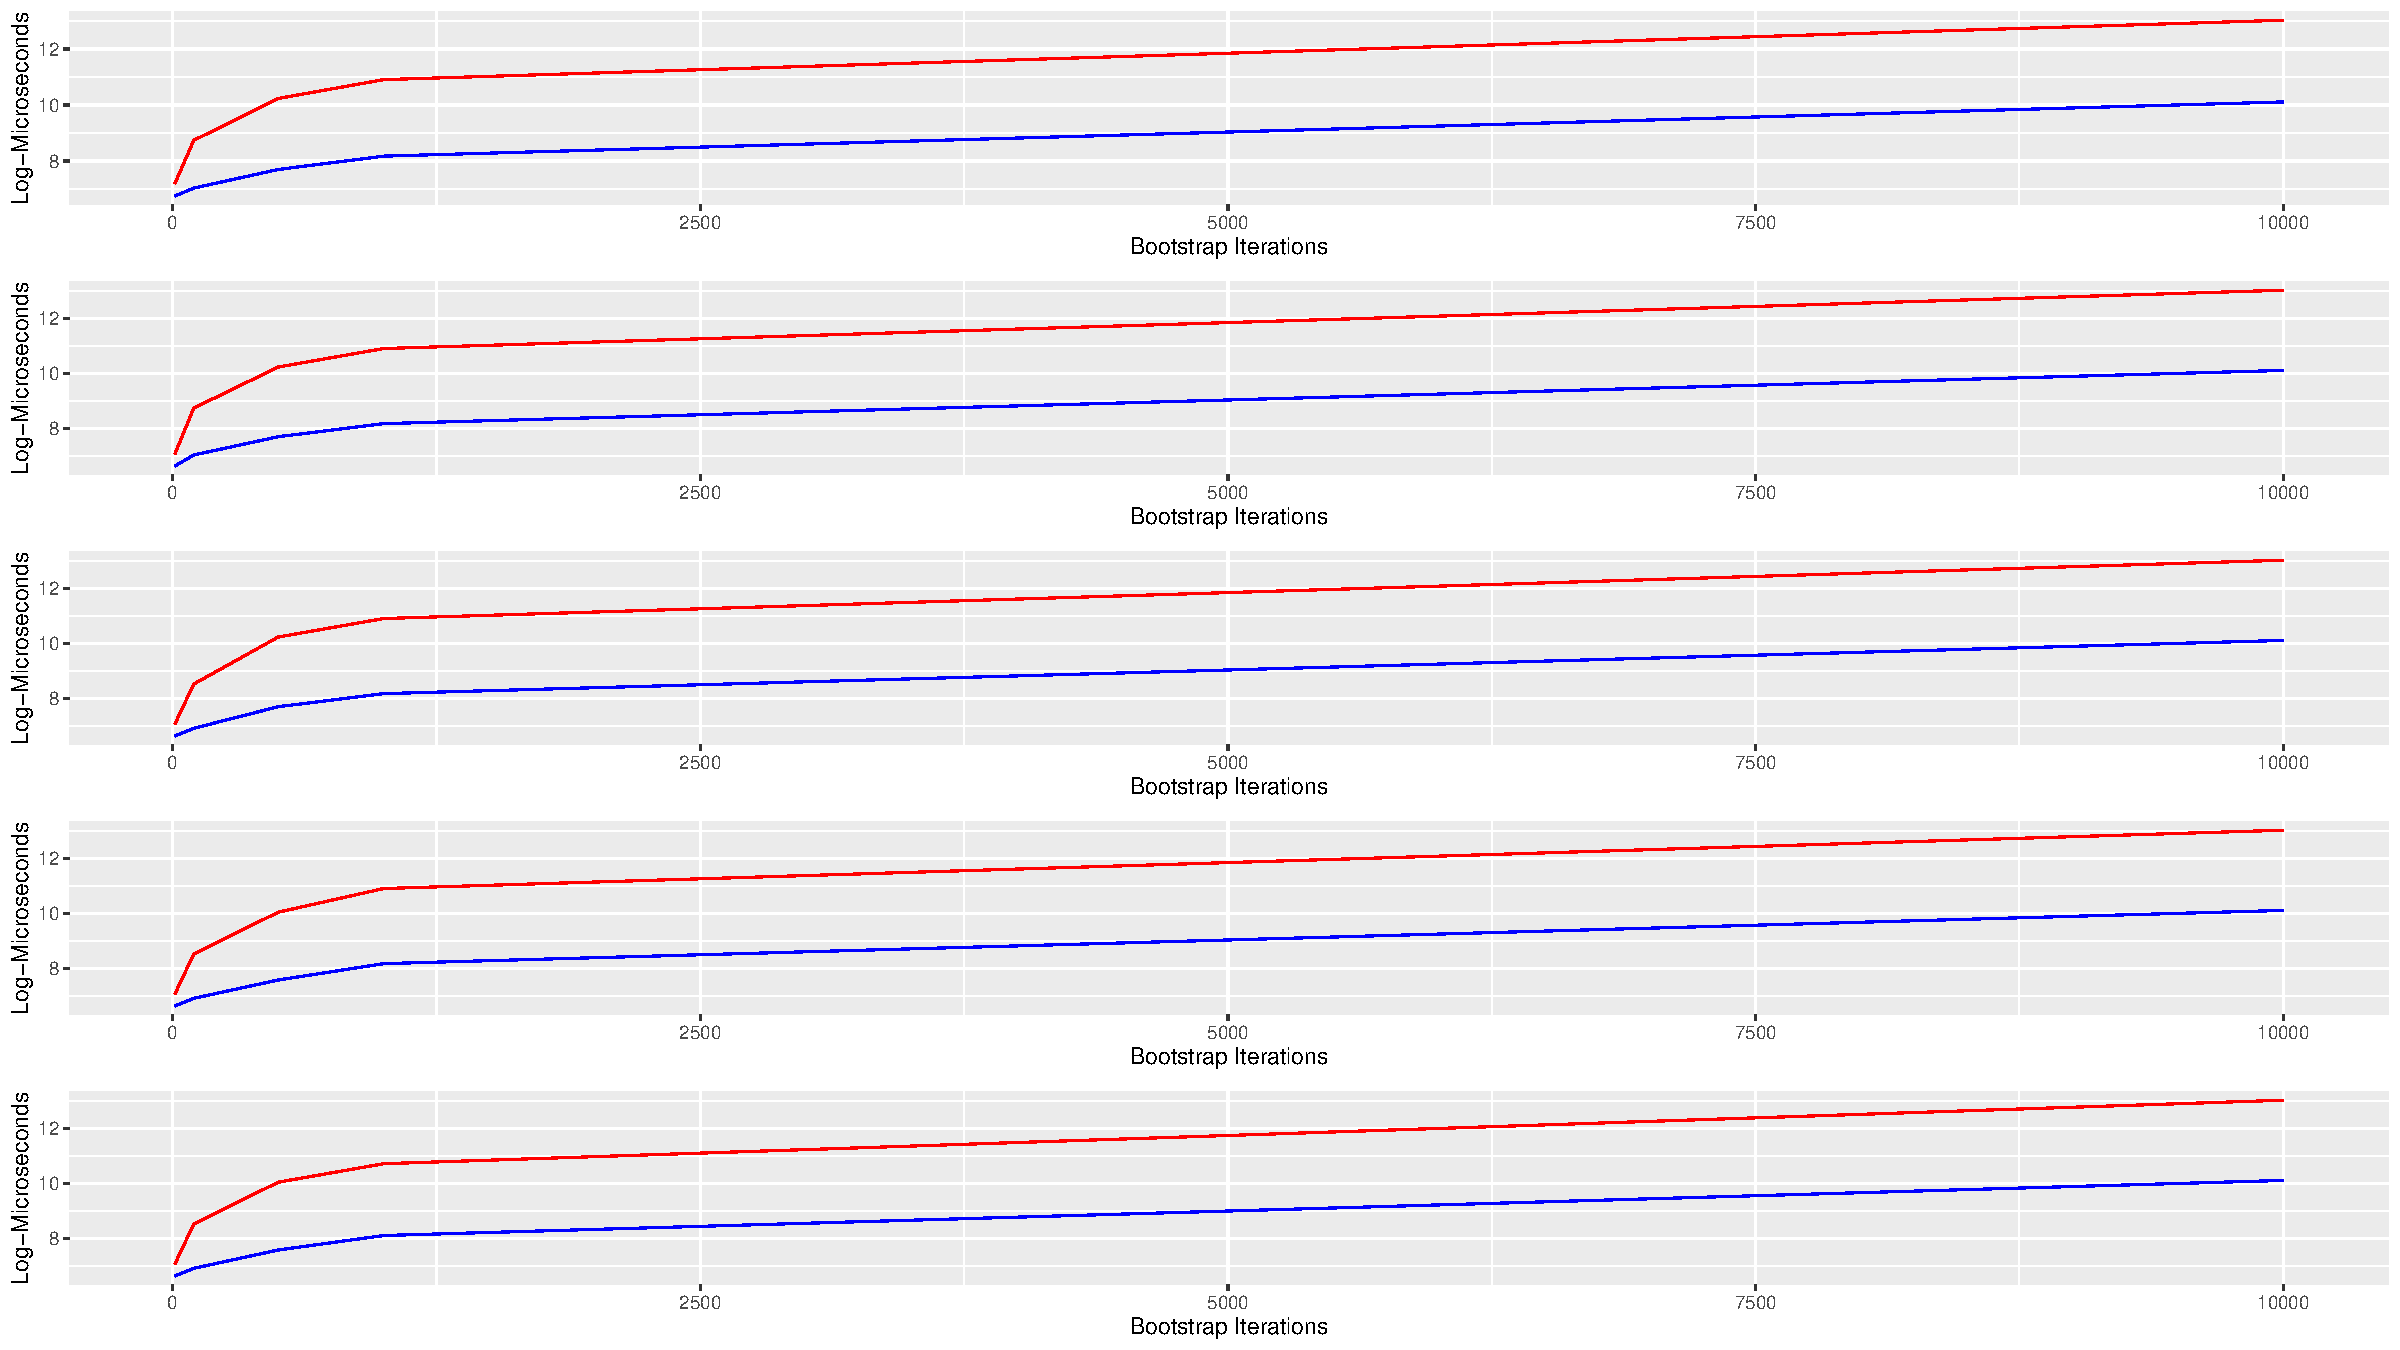
\includegraphics[scale=0.4]{./figures/plot_regression.pdf}
	\caption[Regression Complexity]{Median speed of linear regression: Blue Line: C++, Red Line: R. Each row corresponds to a different sample size from ($5, 10, 50, 100, 200$).}
	\label{fig:regErr}
\end{figure}

\noindent Although the scale is already in log(microseconds) there is a significant difference between those two. The data used for the plot is the median time for each function, for full summary statistics of the time see tables~\ref{reg:time_r} and~\ref{reg:time_cpp} in Appendix B. For both languages the time necessary increases with increased bootstrap iterations, which is only natural. However, even for $10000$ bootstrap iterations C++ is roughly eight times faster than it's R counterpart. Since the simulated problem is of quite simple nature this highlights a huge advantage of lower level languages. We expect that even for more complex linear regression problems (more variables) the computation time increases and that problems which are more complex in their nature themselves would have an even higher advantage in using low level languages (such as generalized linear models from exponential families, classifier problems, dimension reduction techniques) and thus recommend more research in that area.

\subsection{Type-I and -II Errors}
Finally, we want to demonstrate the utility of bootstrap in a specific area: statistical tests. We do this exemplary with the t-test (one and two samples), although we do not show how permutation tests compare to these, which work especially well for two-sample problems. It is noteworthy, that resampling is an important aspect in the field of statistical tests since there exist a large number of research fields where such tests are necessary but suffer from small sample sizes (e.g. translational studies in clinical research). Ideally, a resampled test should reach a Type-I-Error equal to the significance level and also maintain a high power, just as we expect this from a statistical test under large sample situations (or at least asymptotically in theory). Thus, we show Type-I and power for one- and two-sample t-tests with respect to different sample sizes and different bootstrap iterations. 

\begin{figure}
\centering
	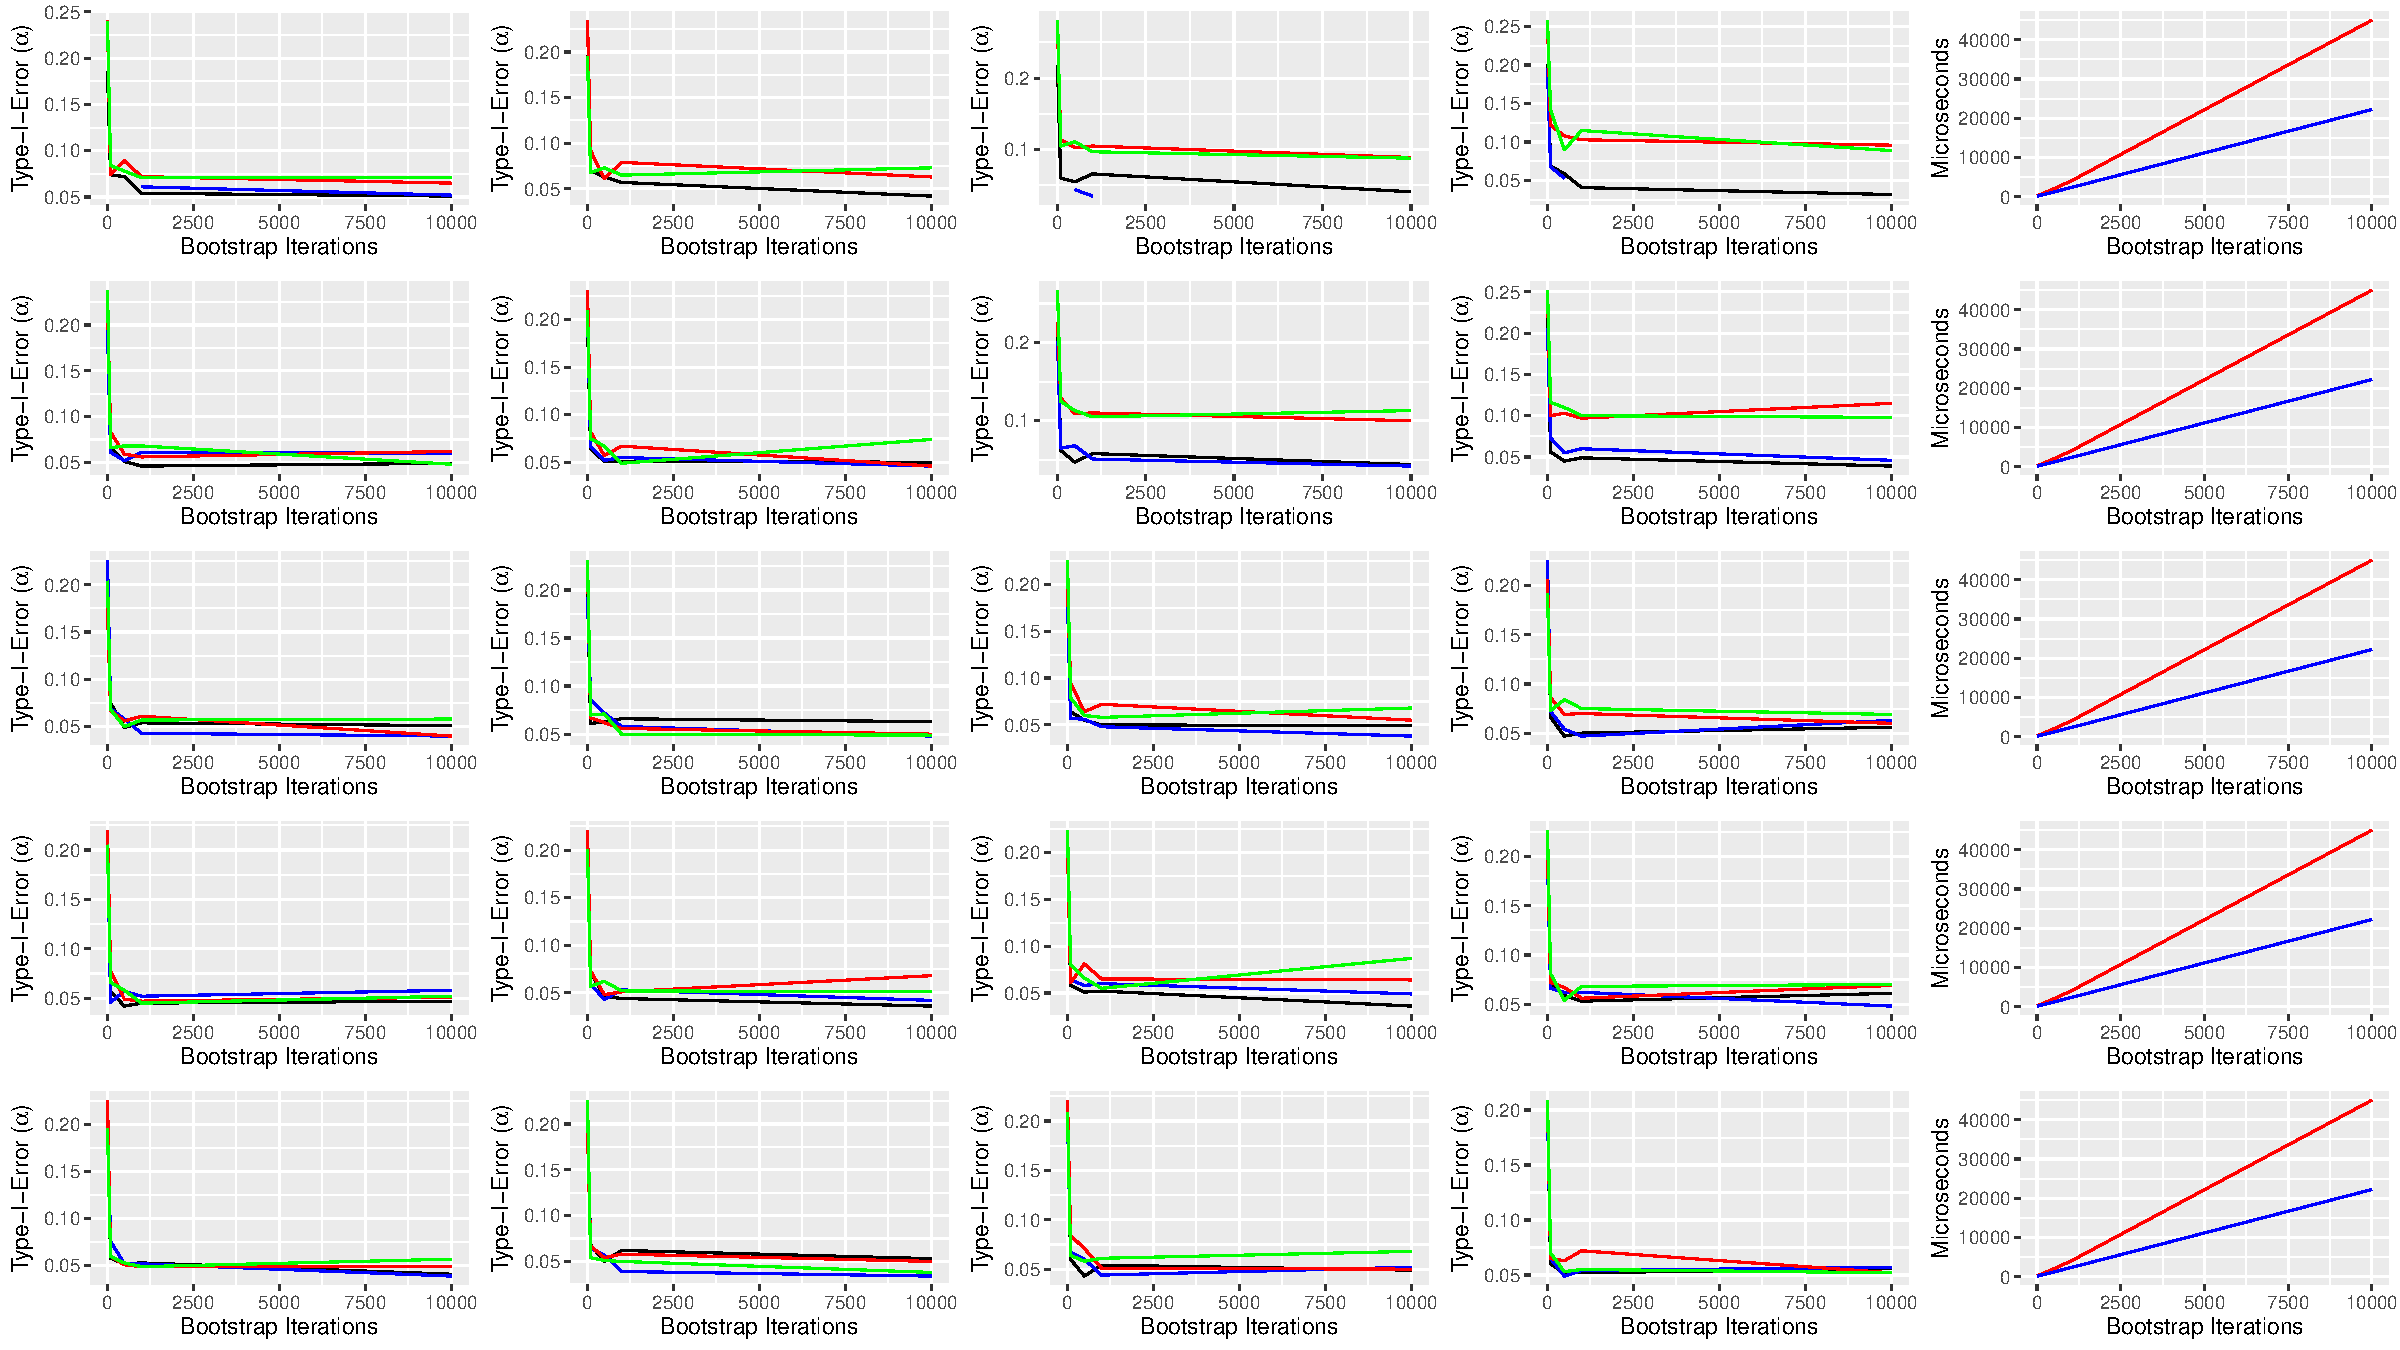
\includegraphics[scale=0.4]{./figures/plot_t1s1.pdf}
	\caption[Type-I-Error One Sample]{Type-1-Error for four different populations in a one-sample setting: Green: $\chi^2$(2), Red: Exp(3), Blue: Pois(5), Black: N(0,1). Each row corresponds to a different sample size from ($5, 10, 50, 100, 200$). The first two columns correspond to the nonparametric bootstrap in R, C++, whereas the third and fourth column correspond to the wild bootstrap in R, C++. The last column depicts the median computation time.}
	\label{fig:t1_s1}
\end{figure}


\begin{figure}
\centering
	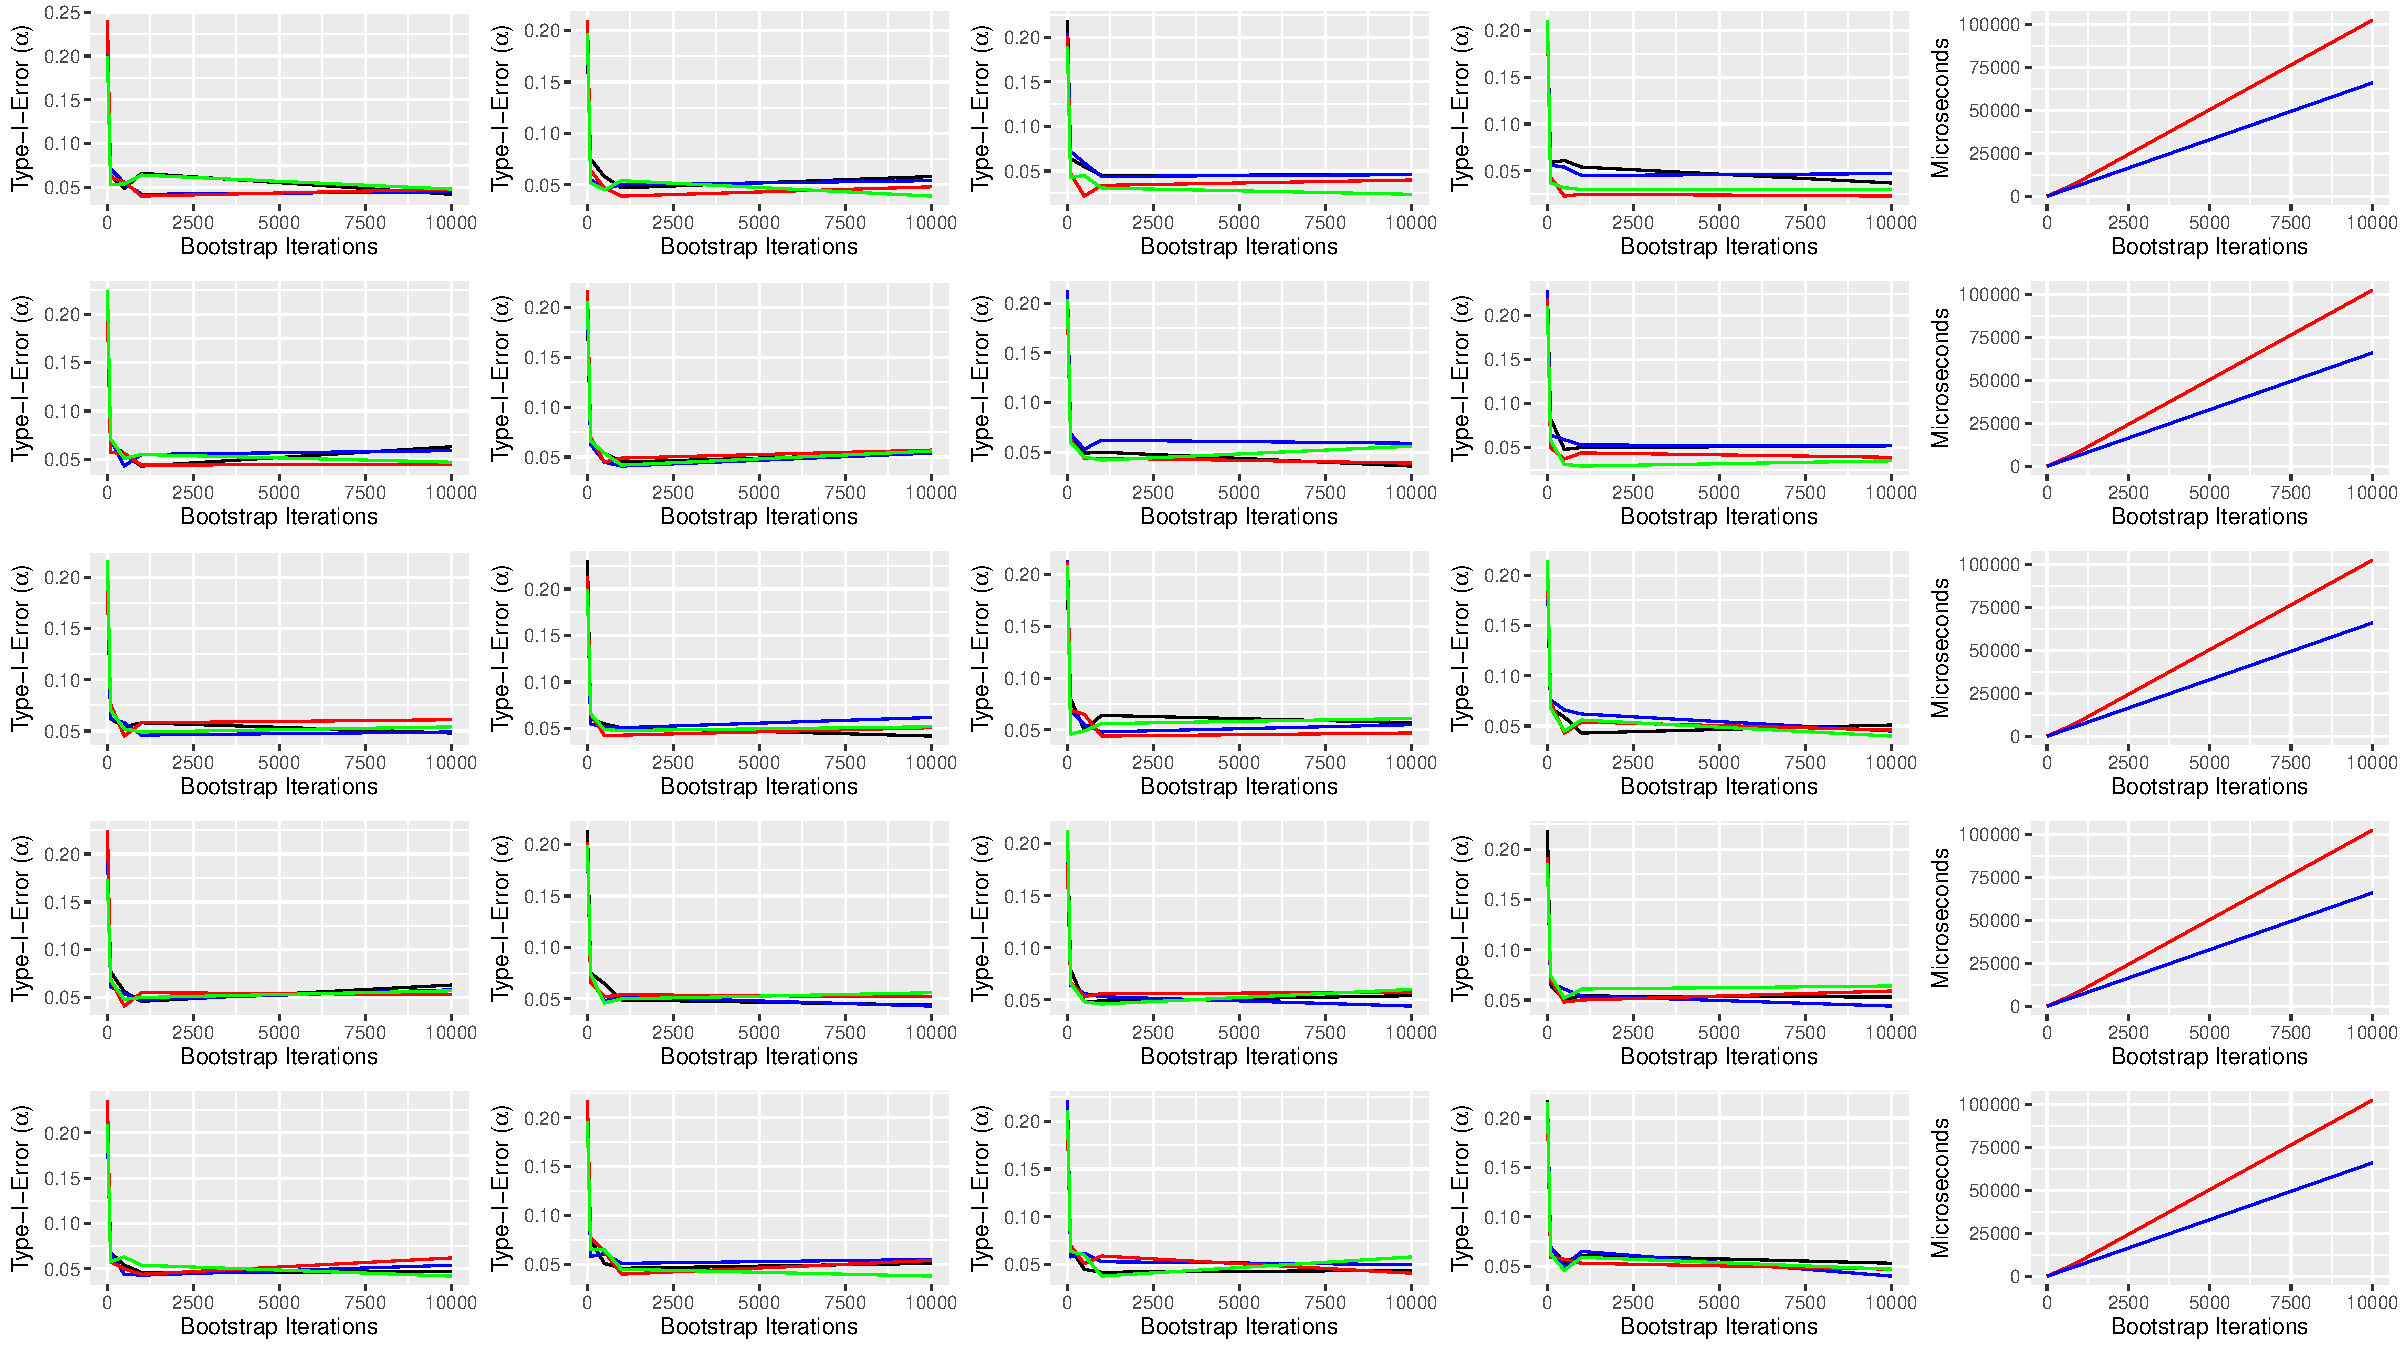
\includegraphics[scale=0.4]{./figures/plot_t1s2.pdf}
	\caption[Type-I-Error Two Sample]{Type-1-Error for four different populations in a two-sample setting: Green: $\chi^2$(2), Red: Exp(3), Blue: Pois(5), Black: N(0,1). Each row corresponds to a different sample size from ($5, 10, 50, 100, 200$). The first two columns correspond to the nonparametric bootstrap in R, C++, whereas the third and fourth column correspond to the wild bootstrap in R, C++. The last column depicts the median computation time.}
	\label{fig:t1_s2}
\end{figure}

\noindent It can be seen in figures~\ref{fig:t1_s1} and~\ref{fig:t1_s2} that the $\chi^2$ and exponential distribution have some struggle to reach the alpha-level, although with increasing sample size they also converge to the significance level. Furthermore, with increasing bootstrap iterations the test converges to the significance level for all samples. Also, the significance level is reached quite fast, raising the question about what should be an ideal number of maximum bootstrap iterations. The figures show that the wild bootstrap performs slightly worse in terms of convergence than the nonparametric bootstrap. It can be seen that in the one-sample case convergence for $\chi^2$ and exponential distribution does not really occur for the first two sample sizes, but do in the two-sample case. A reason for this might be that in the two-sample case two estimators from the same distribution are compared rather than one sample mean against a fixed value. Finally, the computation time is growing linear for both R and C++, but C++ always beats R in the median computation time. As already mentioned before, this is not that important for such trivial problems but can be of high importance for more complex problems. \\
Regarding the power (which can be directly converted to Type-II-Error), the figures~\ref{fig:t2_s1} and~\ref{fig:t2_s2} show the evolution of the power regarding effect size and sample size, all dependend on bootstrap iterations. 

\begin{figure}
 \centering
	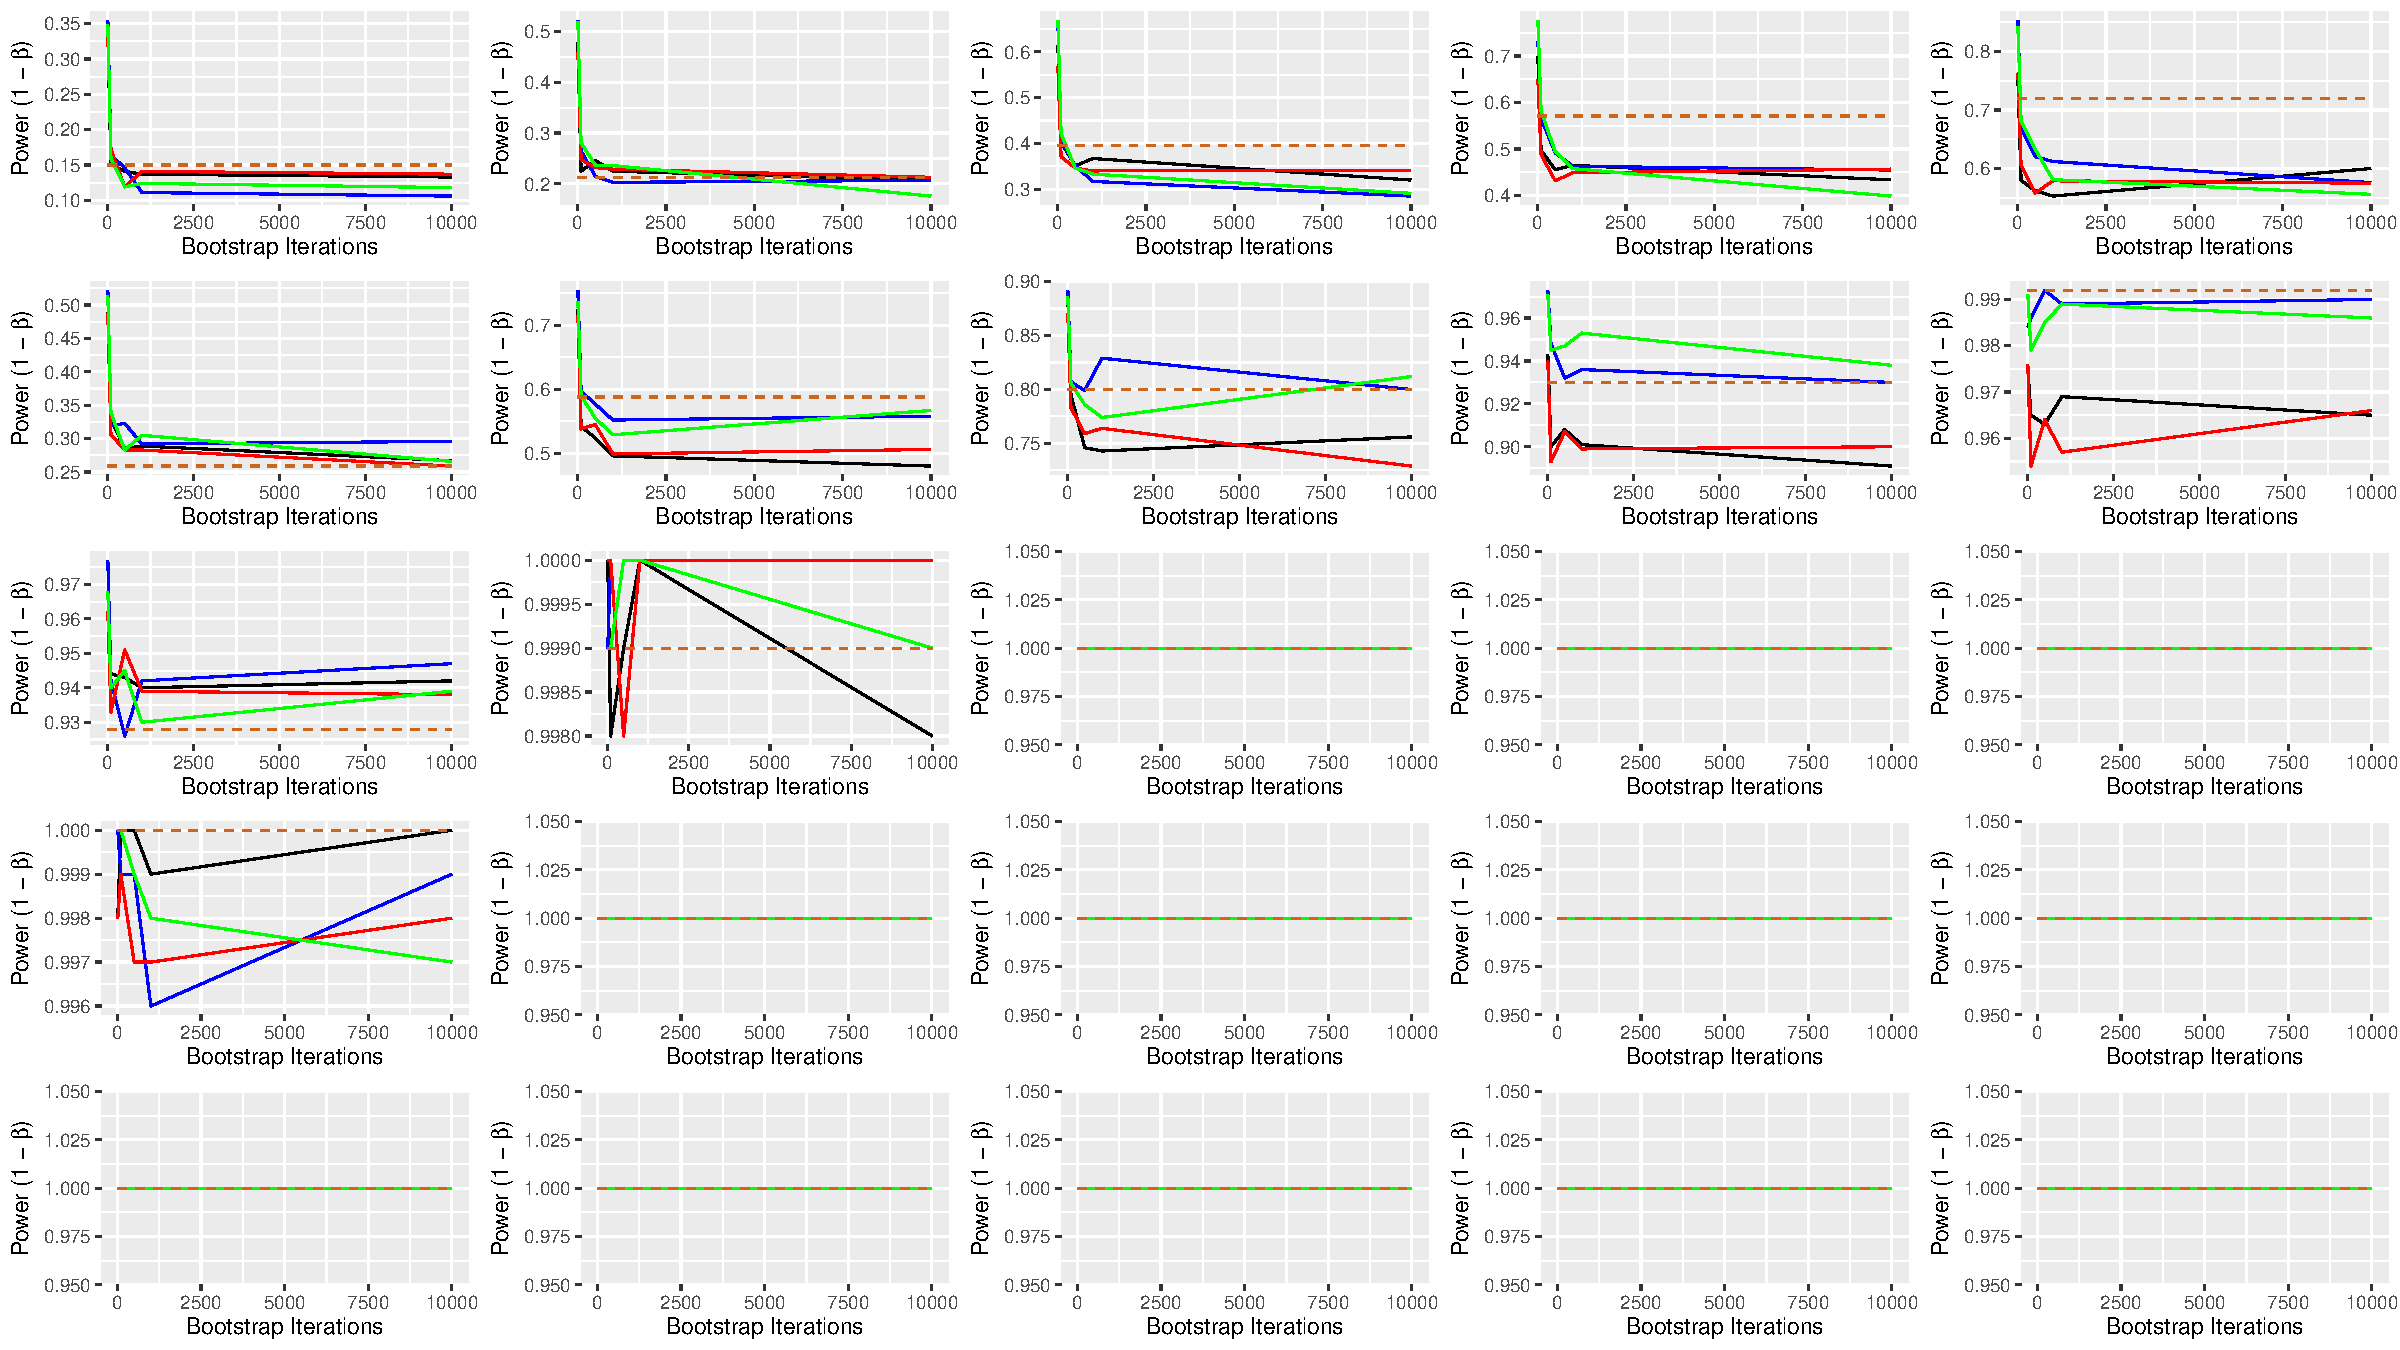
\includegraphics[scale=0.4]{./figures/plot_t2s1.pdf}
	\caption[Power One Sample]{Power for five different population means in a one-sample setting: Black: Nonparametric (R), Blue: Wild (R), Red: Nonparametric (C++), Green: Wild (C++). Each row corresponds to a different sample size from ($5, 10, 50, 100, 200$). Each column corresponds to a different population mean $\mu$ for a normal distribution $N(\mu; \sigma = 1)$, with means $\mathbf{\mu} = (0.5, 0.75, 1, 1.25, 1.5)$ tested against a mean under $H_0$: $\mu_0 = 0$. The dashed brown line refers to a simple t-Test without bootstrap.}
	\label{fig:t2_s1}
\end{figure}


\begin{figure}
\centering
	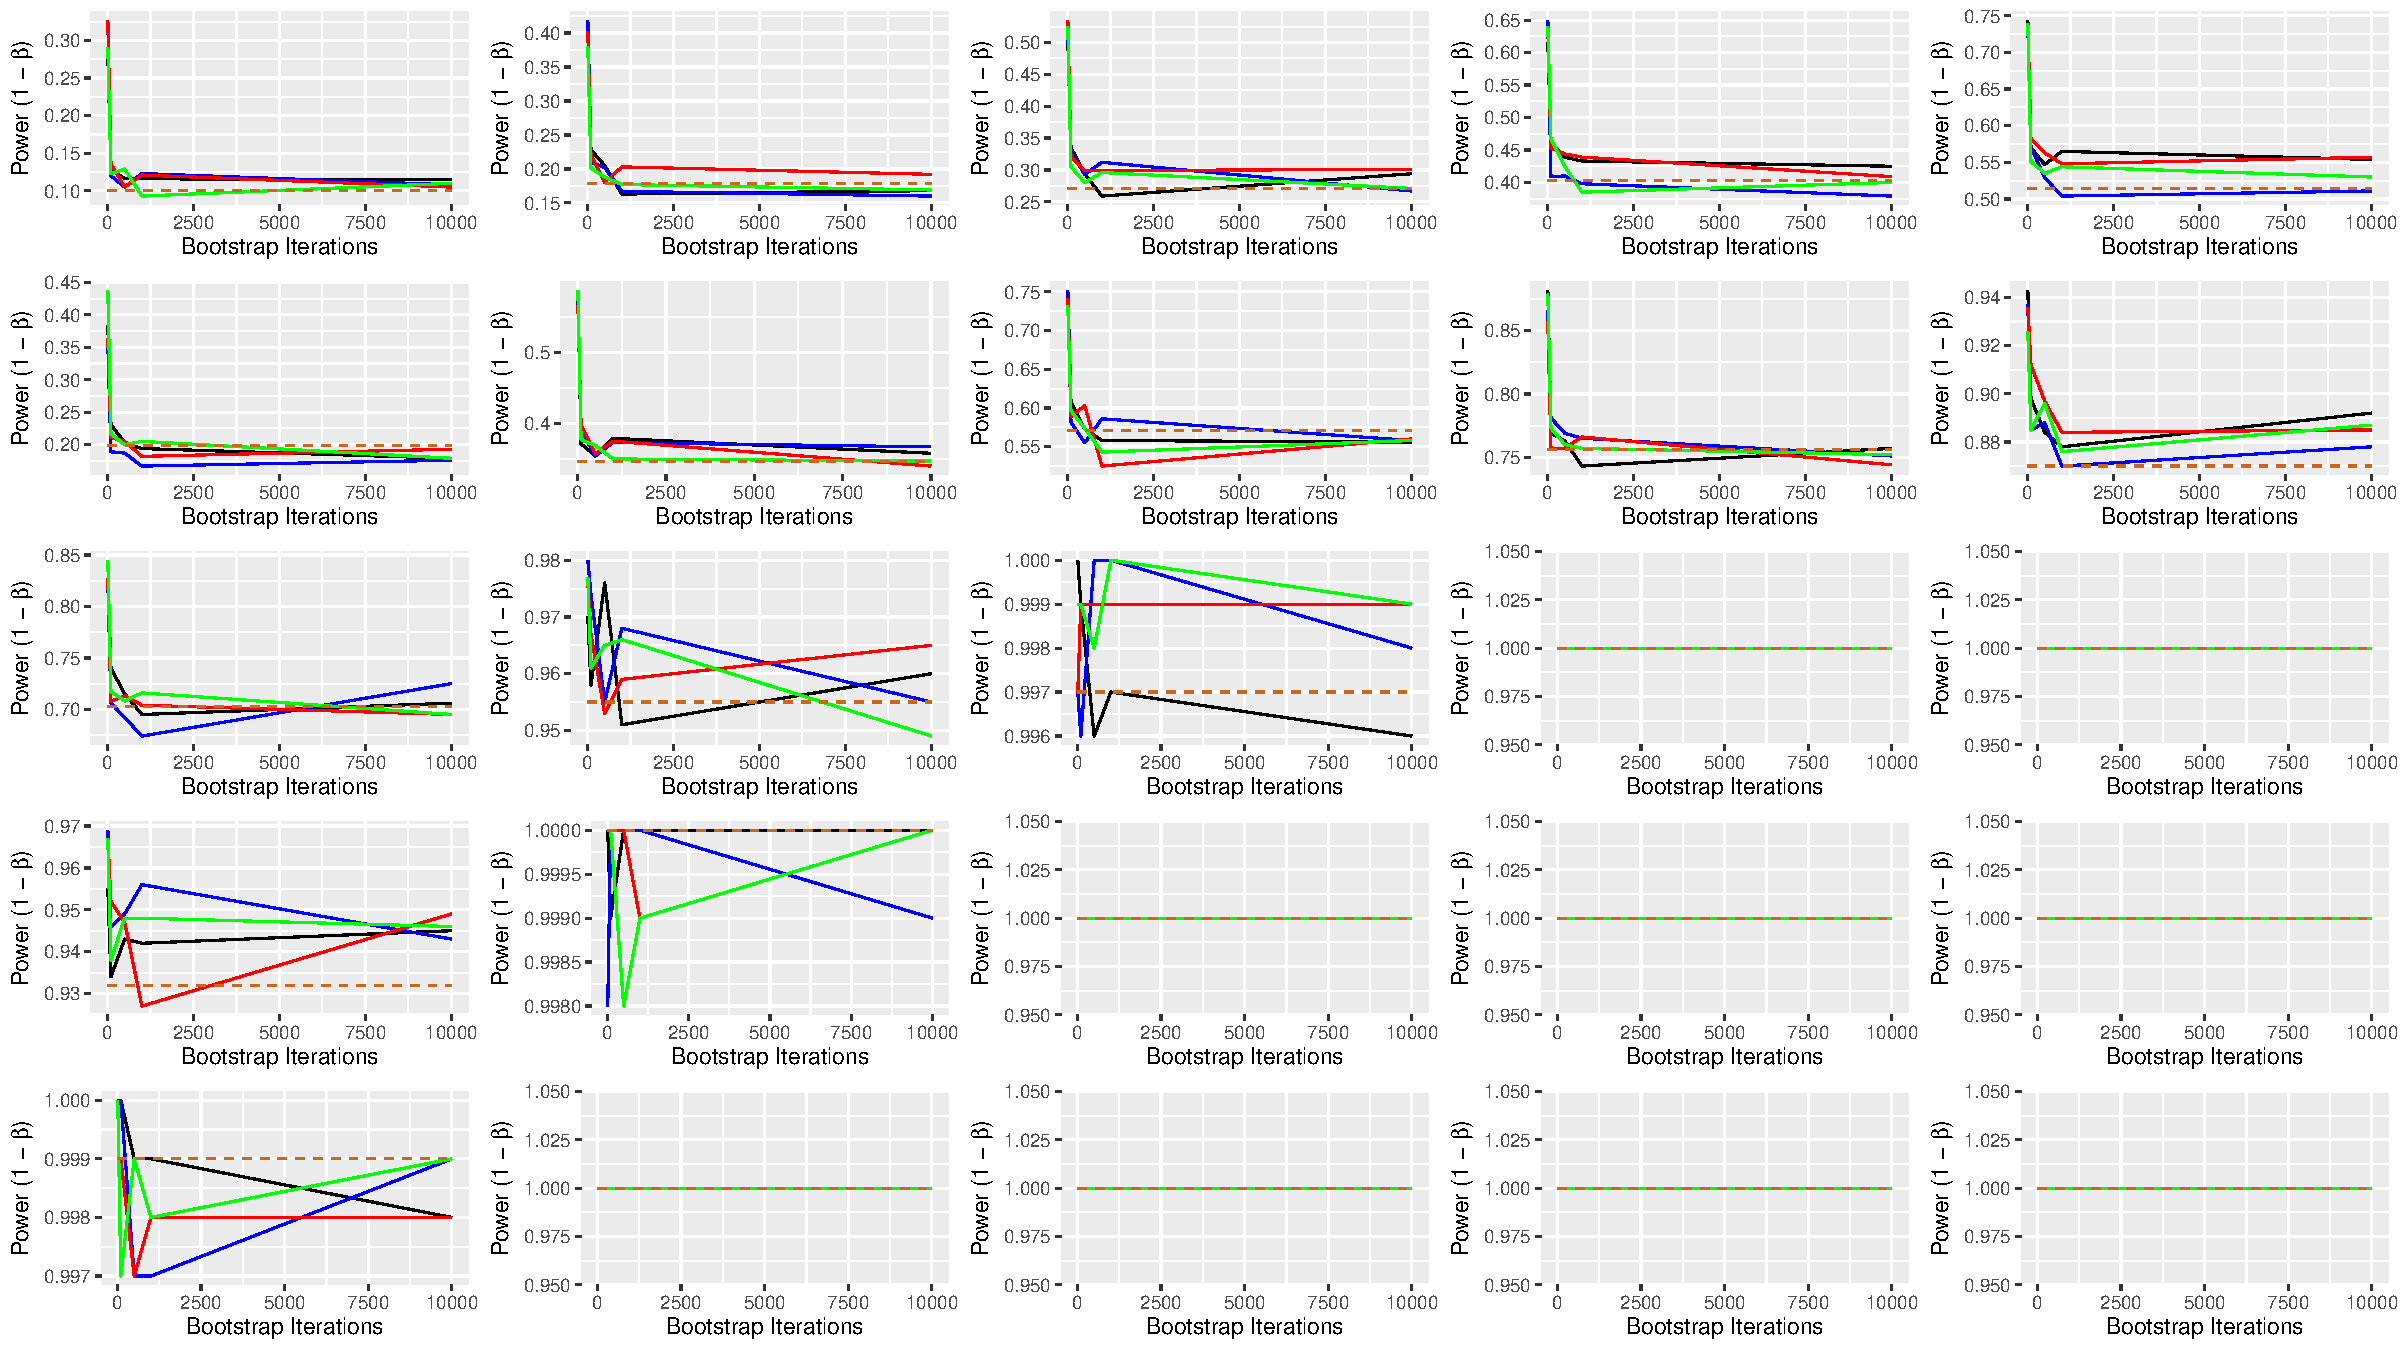
\includegraphics[scale=0.4]{./figures/plot_t2s2.pdf}
	\caption[Power Two Sample]{Power for five different population means in a one-sample setting: Black: Nonparametric (R), Blue: Wild (R), Red: Nonparametric (C++), Green: Wild (C++). Each row corresponds to a different sample size from ($5, 10, 50, 100, 200$). Each column corresponds to a different population mean $\mu$ for a normal distribution $N(\mu; \sigma = 1)$, with means $\mathbf{\mu} = (0.5, 0.75, 1, 1.25, 1.5)$ tested against a $N(0,1)$ population. The dashed brown line refers to a simple t-Test without bootstrap.}
	\label{fig:t2_s2}
\end{figure}

\noindent From the left to right, the power increases, said in other words with an increasing effect size the power increases. This is only natural, since with increasing actual effect size it becomes more unlikely not to reject the null hypothesis. Furthermore, with increasing sample size the power increases very fast, with sample size of $50$ already reporting a power of around $1$ for the first effect size in the one-sample problem and at least $0.7$ for the two-sample problem. However, it should be noted that usually, for such a simple test problem with a sample size of $50$ does not require resampling techniques. There seems to be no systematic difference regarding the different bootstrap techniques or languages.